Mutators that produce type-level mistakes do not necessarily turn
benchmarks into interesting debugging scenarios.

The benchmarks are fully typed, and type checking detects each mistake
at compile time.  Hence, we apply the mutators to versions, dubbed
dubbed{scenarios}, of the benchmarks without some of their type
annotations.  Without the annotations, the type checker may not detect
a mistake at compile time and, instead, the run time checks of the
gradual type system signal an error.  Scenarios with type-level
mistakes that result in run time errors are the ideal ground to
exercise the rational programmer's ability to locate errors.

Specifically, we define an \emph{interesting debugging scenario} as a
scenario that
\begin{enumerate} 
  \item is rejected by the type checker when we restore all its missing type annotations, 
  \item produces a run time error under Erasure as-is, and 
  \item the stack trace of the error mentions at least three distinct components.  
\end{enumerate}

The first criterion simply validates that the debugging scenario concerns
an actual type-level mistake. The second one stipulates that the mistake is
detectable under Erasure to ensure that it is detectable by all three
semantics.   Whether a scenario produces a run time error largely depends on 
the underlying semantics but \citet{gfd-oopsla-2019}
show that a run time error under Erasure implies a run time
error under both Transient and Natural. Thus the criterion aligns
interesting debugging scenarios with our lowest denominator, Erasure, 
and excludes  from consideration the very interesting scenarios indeed where Natural or
Transient can detect a mistake but where Erasure is powerless. Of course this choice favors
Erasure over Transient and Natural and, for the same reason, Transient over
Natural. We consider some form of bias towards one or the other semantics
unavoidable no matter how we define interesting debugging scenarios and we
opt for tipping the scales in favor of the theoretically weakest
semantics. We further discuss the implications of this choice in
section~\ref{sec:discussion}.

The third criterion aims to capture debugging scenarios with a specific
kind of run time error: one produced because of the interaction between the buggy
portion of the program with the rest of the program.  In these cases, the rational programmer
may need to examine several pieces of the program to locate the source of the faulty interaction.
In technical terms, we reliably mark these scenarios by
analyzing the stack trace of a run time error.  If the stack trace mentions at
least two distinct components, then this indicates interaction.  We require a third component because our benchmarks come
with a driver component which is present in the stack trace of all run
time errors. In essence, this last criterion excludes a large number of
trivial to debug, and thus ineffective, scenarios that error immediately when their mutated component is
evaluated. 


%\begin{figure*}
%  \centering
%  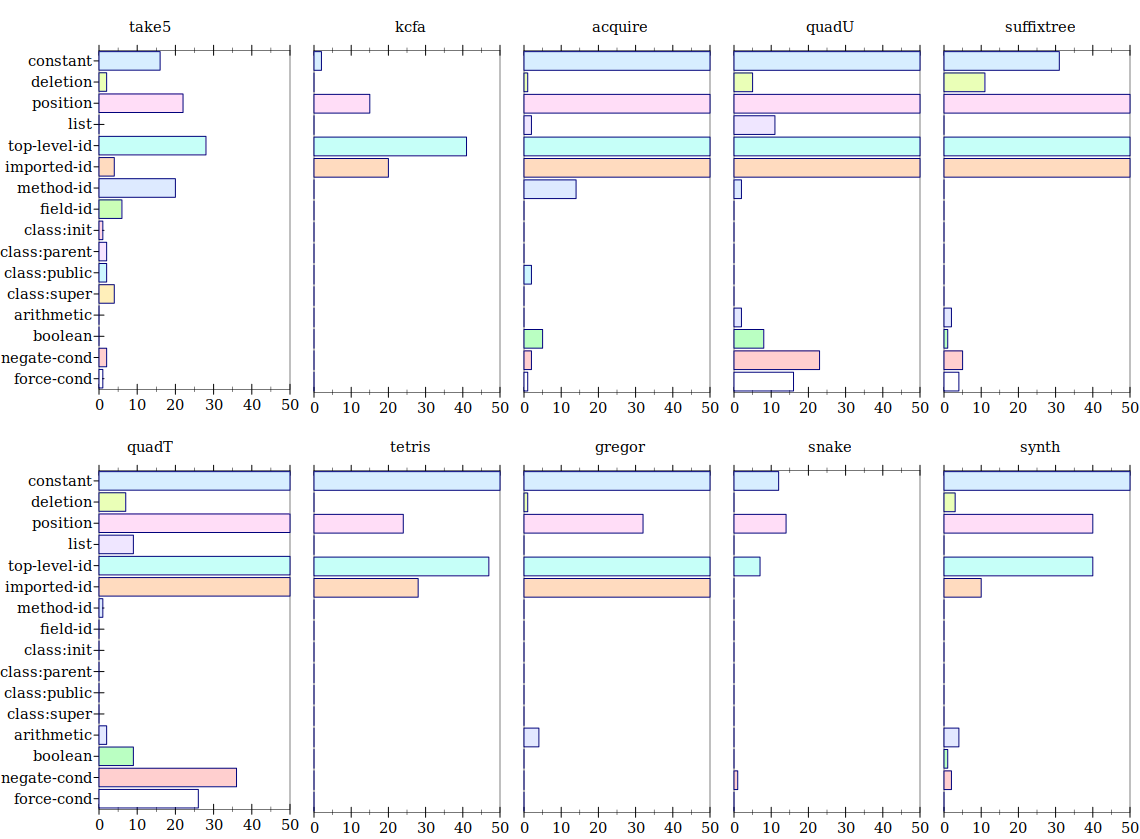
\includegraphics[scale=0.35]{./plots/mutant-breakdown}
%  \caption{Interesting debugging scenarios produced by our mutators. Counts are cut off at 50.}
%  \label{fig:mutant-breakdown}
%\end{figure*}


With the definition of interesting debugging scenarios in hand, we analyze how effective our mutators
are for turning the benchmarks into interesting debugging scenarios.
At a high level, the mutators produce 16,800 mutants with at least one interesting debugging scenario each across all of our benchmarks.
Broken down by benchmark, the mutators produce at least 40 interesting
scenarios for every benchmark, and these scenarios originate from at
least four different mutators per benchmark.  Thus the mutators result in 
a sizeable and diverse population of scenarios for every benchmark.
Furthermore, every mutator contributes scenarios to at least one
benchmark.
That being said, some mutators only apply to a small subset of the benchmarks;
those mutators target specific features which only those benchmarks make us of, so we include them despite their narrow applicability.
For instance, the class-focused mutators are mainly effective in \texttt{take5}, since it is the benchmark with the most extensive use of object-oriented features.
